\chapter{Числа Фибоначчи}

Еще один часто используемый пример в учебниках по программированию это рекурсивная функция,
генерирующая числа Фибоначчи
\footnote{\url{http://go.yurichev.com/17332}}.
Последовательность очень простая: каждое следующее число\EMDASH{}это сумма двух предыдущих.
Первые два числа\EMDASH{}это единицы или 0, 1 и 1.

Начало последовательности:

\begin{center}
$0, 1, 1, 2, 3, 5, 8, 13, 21, 34, 55, 89, 144, 233, 377, 610, 987, 1597, 2584, 4181 ...$
\end{center}

\section{Пример \#1}

Реализация проста. Эта программа генерирует последовательность вплоть до 21.

\lstinputlisting{\CURPATH/fib.c}

\lstinputlisting[caption=MSVC 2010 x86]{\CURPATH/fib.asm}

Этим мы проиллюстрируем стековые фреймы.

\clearpage
Загрузим пример в \olly и дотрассируем до самого последнего вызова функции \ttf{}:

\begin{figure}[H]
\centering
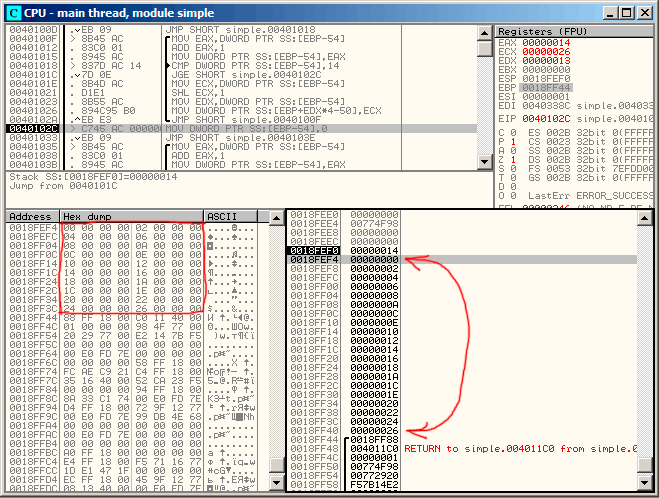
\includegraphics[scale=\FigScale]{\CURPATH/olly.png}
\caption{\olly: последний вызов \ttf{}}
\label{fig:fib_olly}
\end{figure}

\clearpage
Исследуем стек более пристально. 
Комментарии автора книги
\footnote{Кстати, в \olly можно отметить несколько элементов и скопировать их в клипбоард (Ctrl-C).
Это было сделано для этого примера}:

\lstinputlisting{\CURPATH/stack_RU.txt}

Функция рекурсивная
\footnote{т.е. вызывающая сама себя}, 
поэтому стек выглядит как \q{бутерброд}.

Мы видим, что аргумент \IT{limit} всегда один и тот же (\TT{0x14} или 20), но аргументы $a$ и $b$ разные при каждом вызове.

Здесь также адреса \ac{RA} и сохраненные значения \EBP.
\olly способна определять EBP-фреймы, так что она тут нарисовала скобки.
Значения внутри каждой скобки это \gls{stack frame}, иными словами, место, которое каждая
инкарнация функции может использовать для любых своих нужд. 
Можно сказать, каждая инкарнация функции не должна обращаться к элементам стека за пределами
фрейма (не учитывая аргументов функции), хотя это и возможно технически. 
Обычно это так и есть, если только функция не содержит каких-то ошибок.
Каждое сохраненное значение \EBP это адрес предыдущего \gls{stack frame}:
это причина, почему некоторые отладчики могут легко делить стек на фреймы и выводить
аргументы каждой функции.

% TODO add about StackWalk (MSDN)

Как видно, каждая инкарнация функции готовит аргументы для следующего вызова функции.

В самом конце мы видим 3 аргумента функции \main. 
\TT{argc} равен 1 (да, действительно, ведь мы запустили эту программу
без аргументов в командной строке).

Очень легко привести к переполнению стека: просто удалите (или закомментируйте) проверку
предела и процесс упадет с исключением \TT{0xC00000FD} (переполнение стека.)

\section{Пример \#2}

В моей функции есть некая избыточность, так что добавим переменную \IT{next} и заменим на нее
все \q{a+b}:

\lstinputlisting{\CURPATH/fib2.c}

Это результат работы неоптимизирующего MSVC, поэтому переменная \IT{next} действительно
находится в локальном стеке:

\lstinputlisting[caption=MSVC 2010 x86]{\CURPATH/fib2.asm}

\clearpage
Загрузим \olly снова:

\begin{figure}[H]
\centering
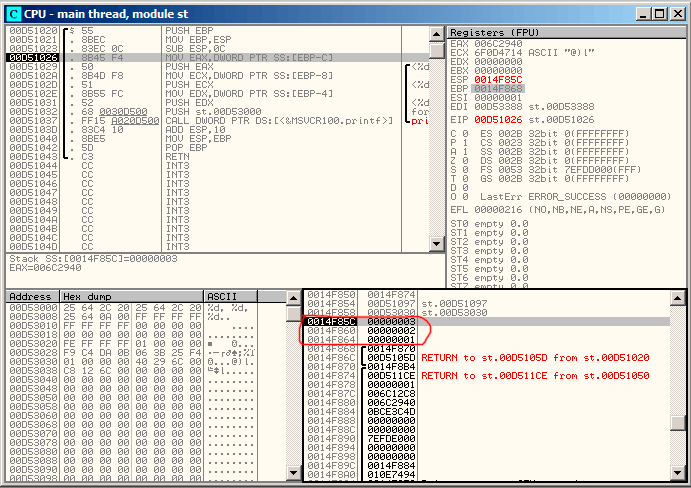
\includegraphics[scale=\FigScale]{\CURPATH/olly2.png}
\caption{\olly: последний вызов \ttf{}}
\label{fig:fib_olly2}
\end{figure}

Теперь переменная \IT{next} присутствует в каждом фрейме.

\clearpage
Рассмотрим стек более пристально. Автор и здесь добавил туда своих комментариев:

\lstinputlisting{\CURPATH/stack2_RU.txt}

% FIXME what a word! hmmm...
Значение переменной \IT{next} вычисляется в каждой инкарнации функции, затем передается
аргумент $b$ в следующую инкарнацию.

\section{Итог}

\label{Recursion_and_tail_call}
\myindex{\Recursion}
Рекурсивные функции эстетически красивы, но технически могут ухудшать производительность
из-за активного использования стека.
Тот, кто пишет критические к времени исполнения участки кода, наверное, должен избегать 
применения там рекурсии.

Например, однажды автор этих строк написал функцию для поиска нужного узла в двоичном дереве. 
Рекурсивно она выглядела очень красиво, но из-за того, что при каждом вызове тратилось время на эпилог и пролог, 
все это работало в несколько раз медленнее чем та же функция, но без рекурсии.

\newcommand{\FnFP}{\footnote{LISP, Python, Lua, \etc{}.}}
\myindex{\Recursion!Tail recursion}
Кстати, поэтому некоторые компиляторы функциональных \ac{PL}\FnFP{} (где рекурсия активно применяется) используют \glslink{tail call}{хвостовую рекурсию}.

